% Validating and Extending a Chapter-Aligned Moodle Engagement Metric
% Compile: pdflatex report.tex (twice)
\documentclass[11pt,a4paper]{article}

\usepackage[T1]{fontenc}
\usepackage[utf8]{inputenc}
\usepackage{lmodern}
\usepackage[margin=2.4cm]{geometry}
\usepackage{amsmath,amssymb}
\usepackage{graphicx}
\usepackage{booktabs}
\usepackage{array}
\usepackage{float}
\usepackage{caption}
\usepackage{subcaption}
\usepackage[round]{natbib}
\usepackage[hidelinks]{hyperref}

\graphicspath{{../outputs/figures/}}

\renewcommand{\figurename}{Fig.}
\captionsetup{font=small,labelfont=bf}
\captionsetup[sub]{font=small}
\setlength{\parskip}{0.35em}
\setlength{\parindent}{1.2em}
\bibliographystyle{plainnat}

\newcommand{\srcnote}{\par\smallskip{\footnotesize\textit{Source: author's analysis of UCL Moodle log data.}}}

\title{\bfseries Validating and Extending a Chapter-Aligned Moodle\\[2pt]
Engagement Metric Across STAT0002 and STAT0004\\[8pt]
\large Evidence from online, hybrid and in-person Moodle delivery cohorts}

\author{Research Internship Report\\
Department of Statistical Science, University College London}
\date{\today}

\begin{document}
\maketitle

\begin{abstract}
\noindent
Virtual learning environments such as Moodle record how students interact with
course materials over time, offering a scalable basis for monitoring online
behavioural engagement. A chapter-aligned, real-time engagement metric was
developed and validated in prior work by \citet{johnston2025}, building on the
course-wide formulation of \citet{chong2019}. This report applies that existing
metric to five module-year cohorts not used in the original validation study,
from STAT0002 and STAT0004 at
University College London, spanning online, hybrid and in-person delivery
periods. The analysis examines association with final grades, the timing of that
association, lower-tail relevance for student support, descriptive comparisons
across delivery conditions, the relative contribution of Frequency, Immediacy and
Diversity, alignment with different assessment components, the incremental value
of temporal regularity, and latent engagement trajectories. Cumulative engagement
is moderately associated with final grade across cohorts (random-effects pooled
$r=0.32$, 95\% CI $[0.25,0.38]$; mixed-effects slope $\approx 3.8$ grade points
per standard deviation). The association is steeper among lower-performing
students, and diagnostic decomposition suggests that breadth of resource use,
promptness and sustained engagement patterns carry more information than raw
activity volume. Latent trajectory classes separate outcomes by roughly 9.7 grade
points between the highest- and lowest-engagement profiles. Delivery condition is
perfectly confounded with academic year and cohort; comparisons across online,
hybrid and in-person deliveries are therefore descriptive, and we find only
limited evidence that delivery condition moderates the engagement--grade
relationship.
\end{abstract}

\noindent\textbf{Keywords:} Moodle engagement; learning analytics; behavioural
engagement; early warning; higher education; STAT0002; STAT0004.

\section{Introduction}
Student engagement---the time and effort students devote to learning
activities---is widely linked to academic performance, satisfaction and
retention. In online and blended higher education, much of the \emph{behavioural}
dimension of engagement can be observed through virtual learning environment
(VLE) log data: which resources students access, how often they return, and how
promptly they engage with newly released material. Moodle and similar platforms
therefore provide an unobtrusive, scalable record of online study behaviour that
is increasingly used in learning analytics and early student support
\citep{henrie2015}.

Institutions nonetheless face a practical tension. Threshold-based early-warning
tools depend on cut-offs that are difficult to justify in advance, while
predictive models often require historical outcome data and may fail to transfer
across cohorts or courses. An alternative is to construct interpretable composite
indicators grounded in engagement theory and computable in real time from log data
alone. \citet{johnston2025} developed such a measure by reconceptualising the
course-wide engagement score of \citet{chong2019} into a weekly, chapter-aligned
formulation based on Frequency, Immediacy and Diversity (F, I, D). Their study
showed that the metric aligns with the retrospective course-wide score from early
in the term, relates to final grades in structured lecture-based modules, and can
help identify low-performing students through engagement quintiles---though with
the modest precision typical of early-warning systems.

This report does not propose a new metric. It applies the existing
chapter-aligned measure to additional cohorts from STAT0002 and STAT0004 and asks
whether the association with final grades holds in a new set of module-year
contexts, whether the signal emerges early enough to inform intervention, whether
it is especially informative for lower-performing students, and whether richer
diagnostic features---Diversity, Immediacy, temporal regularity and trajectory
shape---explain more than raw engagement volume alone. Because STAT0004 spans
online, hybrid and in-person deliveries across different academic years, the
report also offers a descriptive comparison of how the engagement--grade
relationship varies across delivery periods, while treating any such comparison as
non-causal because delivery condition is confounded with cohort and year.

\section{Background and metric context}
Online behavioural engagement refers to observable, sustained interaction with
learning activities in a digital environment. It is only a \emph{proxy} for
learning: Moodle logs capture what happens inside the VLE, not offline study,
in-person attendance or the quality of students' understanding. Even so, when
engagement is measured coherently and validated against academic outcomes, it can
support timely monitoring and targeted support \citep{henrie2015}.

The course-wide metric of \citet{chong2019} combines five indicators---Immediacy,
Frequency, Diversity, Recency and Interval---into a single retrospective score
aggregated across an entire course. That design is useful for end-of-term analysis
but poorly suited to weekly monitoring, and it treats the course as homogeneous
rather than aligned with its chapter structure. \citet{johnston2025} addressed
this by computing Frequency, Immediacy and Diversity separately for each chapter
at each week, min-max scaling each indicator relative to peers at that point in
the term, and summing them into a chapter-level score IDF $= F + I + D$. Chapter
scores are combined across released chapters to yield a cumulative engagement
measure that can be updated as the term progresses without outcome data or model
training. Recency and Interval were excluded because they become unstable when
measured mid-course.

Chapter alignment matters because engagement is most interpretable when measured
in step with how material is released. For early-warning use, practitioners also
need to understand the recall--precision trade-off: flagging the lowest-engagement
students may capture many who ultimately struggle, but also many who would have
succeeded without intervention \citep{conijn2017}. The present report takes the
metric definition as given and focuses on how it behaves on new UCL cohorts and
what additional diagnostic insight can be extracted from its components and
related temporal patterns.

\section{Data}
The analysis uses five module-year deliveries from two undergraduate statistics
modules at University College London. STAT0002 is a first-year foundations module
represented here by an online cohort (2020--21) and an in-person cohort
(2022--23). STAT0004 is a second-year module and the only module in this dataset
spanning all three delivery conditions: online (2020--21), hybrid (2021--22) and
in-person (2022--23). Each delivery covers eleven teaching weeks with up to ten
labelled chapters. Final grades are recorded on a 0--100 scale; grades below 50
indicate low performance (D/F), and below 40 indicate failure (F). Students with
a recorded grade of zero, typically reflecting exam absence, were excluded.

Table~\ref{tab:inventory} summarises the cohorts. The main engagement--grade
sample comprises $N=1{,}291$ students with both engagement records and valid
final grades after exclusions. The latent trajectory analysis below uses
$N=1{,}290$ students with complete weekly engagement profiles suitable for class
assignment; the difference of one student reflects missing weekly coverage in
the trajectory model, not an error in the cohort inventory.

\begin{table}[H]
\centering
\caption{Cohort inventory for the main engagement--grade sample ($N=1{,}291$).}
\label{tab:inventory}
\small
\begin{tabular}{lllrrrr}
\toprule
Module & Year & Condition & $N$ & Mean (SD) & \%\,$<50$ & \%\,$<40$ \\
\midrule
STAT0002 & 2020--21 & Online    & 342 & 66.8 (13.8) & 9.9  & 1.8 \\
STAT0002 & 2022--23 & In-person & 268 & 67.4 (13.0) & 10.4 & 2.6 \\
STAT0004 & 2020--21 & Online    & 312 & 62.7 (12.2) & 12.5 & 2.9 \\
STAT0004 & 2021--22 & Hybrid    & 172 & 71.9 (8.8)  & 1.7  & 0.0 \\
STAT0004 & 2022--23 & In-person & 197 & 70.6 (11.3) & 3.6  & 1.0 \\
\midrule
\multicolumn{3}{l}{\textbf{Total}} & \textbf{1{,}291} & & & \\
\bottomrule
\end{tabular}
\srcnote
\end{table}

Two design features constrain interpretation. First, the share of low-performing
students varies widely across cohorts (from 1.7\% to 12.5\%), which limits how
sharply any early-warning flag can perform in the highest-achieving deliveries.
Second, delivery condition is \textbf{perfectly confounded} with academic year and
cohort: online corresponds to 2020--21, hybrid to 2021--22, and in-person to
2022--23. Comparisons across conditions therefore describe different module-year
contexts rather than randomly assigned delivery modes, and no causal claim about
online, hybrid or in-person delivery can be supported.

The modules also differed in assessment structure. STAT0002 in-person records
separate exam, participation and peer-marking components; STAT0004 deliveries
include coursework and quiz marks, with a group component in the in-person year.
This matters because Moodle engagement may align more closely with
individual or exam-style assessment than with group, peer-marked or participation
components. Where component marks were available, this report therefore analyses
whether the engagement metric correlates more strongly with individually assessed
work than with collaborative or peer-assessed components.

\section{Engagement feature construction}
Weekly chapter-level contribution values were available for each student. These
values are stored as \emph{per-week increments}, not as cumulative totals. For
each student and week, contributions were summed across chapters to obtain weekly
Frequency, Immediacy and Diversity totals. The weekly composite was then defined
additively as
\[
\mathrm{IDF}_\mathrm{week} = \mathrm{freq}_\mathrm{week} +
\mathrm{imm}_\mathrm{week} + \mathrm{div}_\mathrm{week},
\]
and cumulative measures were obtained by summing across weeks:
$\mathrm{cum\_freq}$, $\mathrm{cum\_imm}$, $\mathrm{cum\_div}$ and
$\mathrm{cum\_IDF}$. This additive definition matches the chapter-level
formulation of \citet{johnston2025}; it is not a multiplicative composite. A
reconstruction check confirmed that the supplied contributions are consistent
with the intended Frequency and Diversity definitions.

For extension analyses, additional timing and regularity features were derived
from event logs (for example, variation in weekly activity and gaps between
sessions). Latent-class mixed models were also fitted to normalised weekly
cumulative IDF curves to identify distinct engagement trajectories over the term.

\section{Methods}

\subsection{Association between engagement and final grade}
Within each cohort, Spearman rank correlations were computed between cumulative
engagement and final grade at each week and at the end of term. To synthesise
evidence across cohorts, cohort-specific correlations were pooled using a
random-effects meta-analysis, reporting the pooled correlation, confidence
interval and $I^2$ heterogeneity statistic. Complementing rank-based evidence, a
mixed-effects model was fitted with final grade as the outcome and standardised
cumulative IDF as the predictor, allowing the slope to vary by cohort. This
expresses the association on the grade scale in points per one standard deviation
of engagement.

\subsection{Timing and early-course usefulness}
Weekly Spearman correlations between cumulative engagement and final grade were
tracked across the term to assess how early the association emerges. For each
cohort, a bootstrap procedure identified the earliest week at which the
correlation was statistically indistinguishable from its end-of-term value,
providing a practical sense of when the signal stabilises.

\subsection{Lower-tail and early-warning analysis}
Students were grouped into engagement quintiles at selected weeks, and the
distribution of final grades within each quintile was examined. Quantile
regression estimates the relationship between engagement and final grade at
different points in the grade distribution---for example, among the lowest 10\%
of performers rather than only at the median---so that one can ask whether the
metric matters more for students already at academic risk. Particular attention
was given to the lower tail ($\tau=0.1$) relative to the median ($\tau=0.5$).
For early-warning relevance, the bottom engagement quintile was treated as a
risk flag and evaluated using the area under the ROC curve (AUC), recall and
precision for identifying students scoring below 50\% at the end of term.

\subsection{Diagnostic decomposition of engagement}
Frequency, Immediacy and Diversity are strongly correlated, so ordinary
regression coefficients do not reveal which dimension carries unique information.
Variance inflation factors were examined to confirm collinearity, and the LMG
relative-importance decomposition was used to partition explained variance among
the three indicators in a way that is stable under collinearity: it averages each
predictor's contribution to $R^2$ over all possible orderings in which the
indicators enter the model.

\subsection{Assessment-component validity}
Where separate assessment marks were available, engagement was correlated with
each component and Steiger's test for dependent correlations was used to compare
whether engagement aligns more strongly with individually assessed work (exams,
quizzes) than with group- or peer-marked components.

\subsection{Temporal regularity and trajectory analysis}
Timing and regularity features were added to models already containing F, I and
D to test whether \emph{how} students engage over time adds information beyond
\emph{how much} and \emph{how broadly} they engage. Separately, latent-class mixed
models were applied to weekly cumulative IDF profiles to identify groups of
students following distinct engagement trajectories and to compare their final
grades. This treats students' weekly engagement profiles as trajectories and groups
students with similar shapes of engagement over time, rather than only comparing
their final cumulative engagement score.

\subsection{Robustness checks}
The main conclusions were examined under degree-programme adjustment,
false-discovery-rate correction using the Benjamini--Hochberg procedure across
weekly association tests, alternative bounded outcome specifications, and
variation in the at-risk engagement threshold. These
checks were kept brief and interpreted in the context of the primary findings
rather than treated as a separate technical audit.

\section{Results}

\subsection{Engagement is moderately associated with final grades across cohorts}
Across all five cohorts, cumulative engagement is positively and moderately
associated with final grade. The random-effects pooled rank correlation for
cumulative IDF at week 11 is $r=0.32$ (95\% CI $[0.25, 0.38]$), with
low-to-moderate heterogeneity across cohorts ($I^2=39\%$). Frequency, Immediacy
and Diversity show similar pooled associations when analysed separately
(Table~\ref{tab:meta}). On the grade scale, the mixed-effects estimate
corresponds to approximately 3.8 grade points per one standard deviation increase
in engagement. Figure~\ref{fig:forest} shows that every cohort lies above zero,
but the association is far from perfect prediction---engagement is a useful but
imperfect proxy for academic performance.

\begin{table}[H]
\centering
\caption{Pooled rank correlations and mixed-effects slopes at week 11.}
\label{tab:meta}
\small
\begin{tabular}{lcccc}
\toprule
Indicator & Pooled $r$ [95\% CI] & $I^2$ & Slope (SE) & Moderator $p$ \\
\midrule
Frequency & 0.28 [0.22, 0.34] & 27\% & 3.36 (0.53) & 0.92 \\
Immediacy & 0.30 [0.24, 0.37] & 37\% & 3.63 (0.58) & 0.88 \\
Diversity & 0.31 [0.24, 0.37] & 33\% & 3.62 (0.53) & 0.87 \\
\textbf{IDF} & \textbf{0.32 [0.25, 0.38]} & \textbf{39\%} & \textbf{3.79 (0.58)} & 0.89 \\
\bottomrule
\end{tabular}
\srcnote
\end{table}

\begin{figure}[H]
\centering
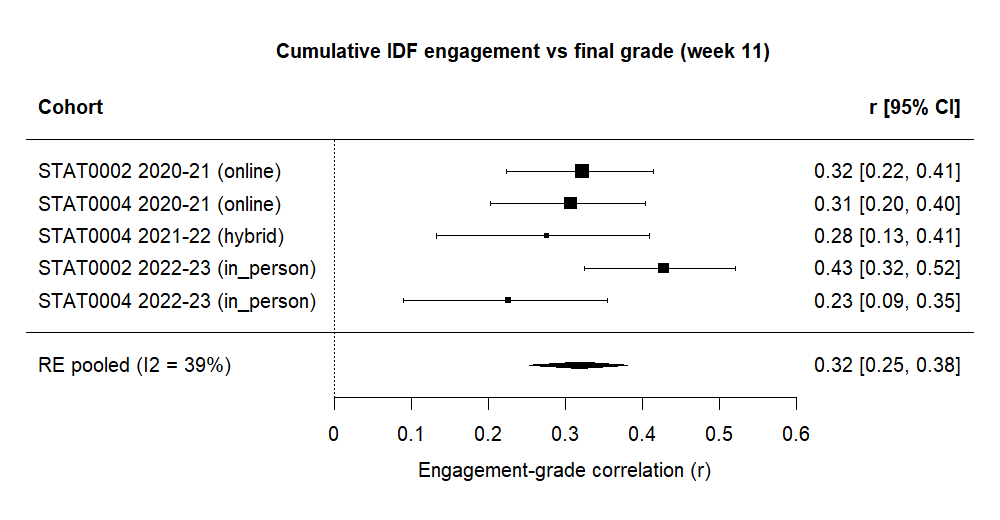
\includegraphics[width=0.82\textwidth]{12_forest_IDF.png}
\caption{Cohort-specific and pooled week-11 correlations between cumulative IDF
engagement and final grade. All cohorts show positive associations; the
random-effects estimate summarises the overall moderate engagement--grade
relationship.}
\label{fig:forest}
\end{figure}

\subsection{The signal appears early but not identically across cohorts}
The engagement--grade association is visible from the early weeks of the term in
most cohorts. Bootstrap stabilisation analysis indicates that the weekly
correlation reaches its end-of-term level by week 1 or 2 in four of the five
deliveries (Table~\ref{tab:stab}, Figure~\ref{fig:stab}). In those cohorts the
signal is relatively flat across the term, so stabilisation occurs almost
immediately. STAT0002 in-person is the exception: the correlation strengthens
steadily and stabilises only around week 9, by which point it has become the
strongest cohort-level association ($r \approx 0.41$). In practical terms, the
metric already carries substantial information by the course midpoint in most
deliveries, but the timing of stabilisation depends on how the signal accrues over
the term.

\begin{table}[H]
\centering
\caption{Stabilisation week and end-of-term IDF--grade correlation.}
\label{tab:stab}
\small
\begin{tabular}{lcc}
\toprule
Cohort & Stabilisation week & End-of-term $r$ \\
\midrule
STAT0002 online    & 2 & 0.28 \\
STAT0002 in-person & 9 & 0.41 \\
STAT0004 online    & 1 & 0.30 \\
STAT0004 hybrid    & 1 & 0.23 \\
STAT0004 in-person & 1 & 0.19 \\
\bottomrule
\end{tabular}
\srcnote
\end{table}

\begin{figure}[H]
\centering
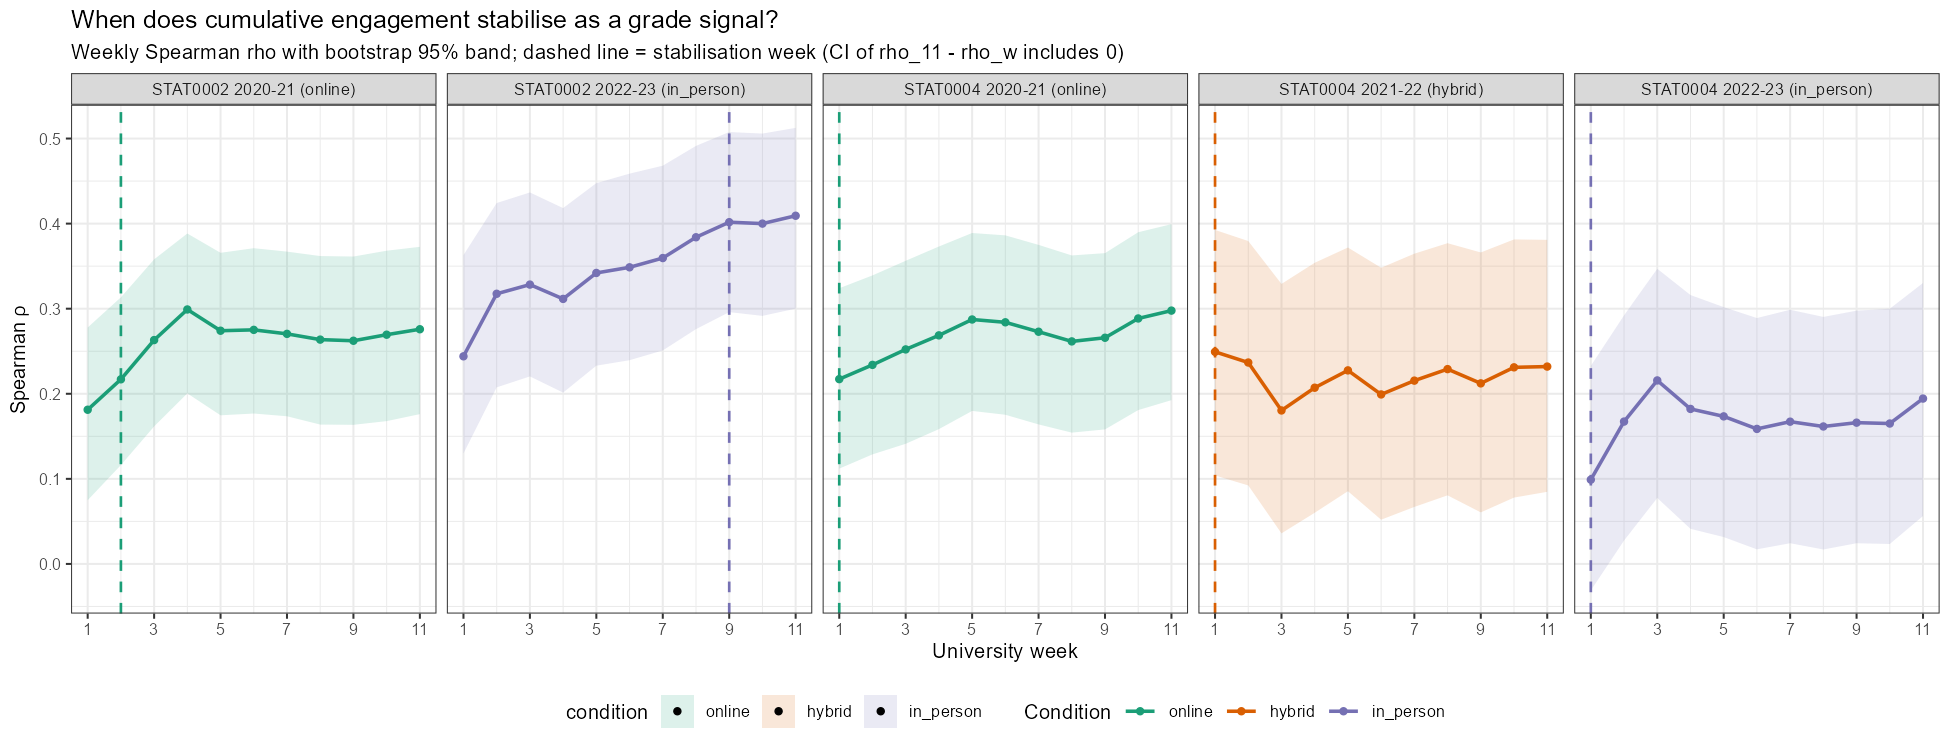
\includegraphics[width=0.92\textwidth]{15_stabilisation.png}
\caption{Weekly Spearman correlation between cumulative engagement and final grade
by cohort, with bootstrap stabilisation week marked. Most cohorts reach their
end-of-term association level within the first two weeks; STAT0002 in-person
shows a strengthening signal that stabilises around week~9.}
\label{fig:stab}
\end{figure}

\subsection{Lower engagement groups tend to have lower grades}
When students are ranked by cumulative engagement and grouped into quintiles,
final grades tend to rise across successive quintiles, particularly in STAT0002,
where quintile separation is clearest (Figure~\ref{fig:quintile}). At weeks 3 and 6,
lowest-engagement quintile is the group whose grade distribution most often
approaches or crosses the 50\% low-performance threshold, while the
highest-engagement quintile consistently shows the strongest outcomes. Separation
between adjacent middle quintiles is weaker, which is consistent with a monotone
but noisy relationship rather than sharp boundaries between moderate engagement
levels.

\begin{figure}[H]
\centering
\includegraphics[width=0.95\textwidth]{06_quintile_boxplots_w3_w6.png}
\caption{Final-grade distributions by engagement quintile at weeks 3 and 6.}
\label{fig:quintile}
\end{figure}

\subsection{Engagement is especially informative in the lower grade tail}
Quantile regression shows that the engagement--grade slope is steeper in the lower
tail of the grade distribution than at the median in every cohort
(Table~\ref{tab:quantile}, Figure~\ref{fig:quantile}). On average, the slope at
$\tau=0.1$ exceeds the median slope by about 2.3 grade points per standard
deviation of engagement. This pattern suggests that variation in engagement is
most consequential among students at greater academic risk, while mattering less
for students who are already performing strongly---a property that supports the
metric's relevance for early support, even though operational flagging still
faces modest precision.

\begin{table}[H]
\centering
\caption{Quantile-regression slopes (grade points per +1 SD cumulative IDF).}
\label{tab:quantile}
\small
\begin{tabular}{lcccc}
\toprule
Cohort & $\tau=0.1$ & $\tau=0.5$ & $\tau=0.9$ & $\tau_{0.1}-\tau_{0.5}$ \\
\midrule
STAT0002 online    & 5.32 & 3.22 & 2.58 & 2.11 \\
STAT0002 in-person & 7.88 & 5.04 & 2.96 & 2.84 \\
STAT0004 online    & 6.06 & 3.15 & 2.17 & 2.91 \\
STAT0004 hybrid    & 3.26 & 2.66 & 1.34 & 0.59 \\
STAT0004 in-person & 3.97 & 1.10 & 1.28 & 2.88 \\
\bottomrule
\end{tabular}
\srcnote
\end{table}

\begin{figure}[H]
\centering
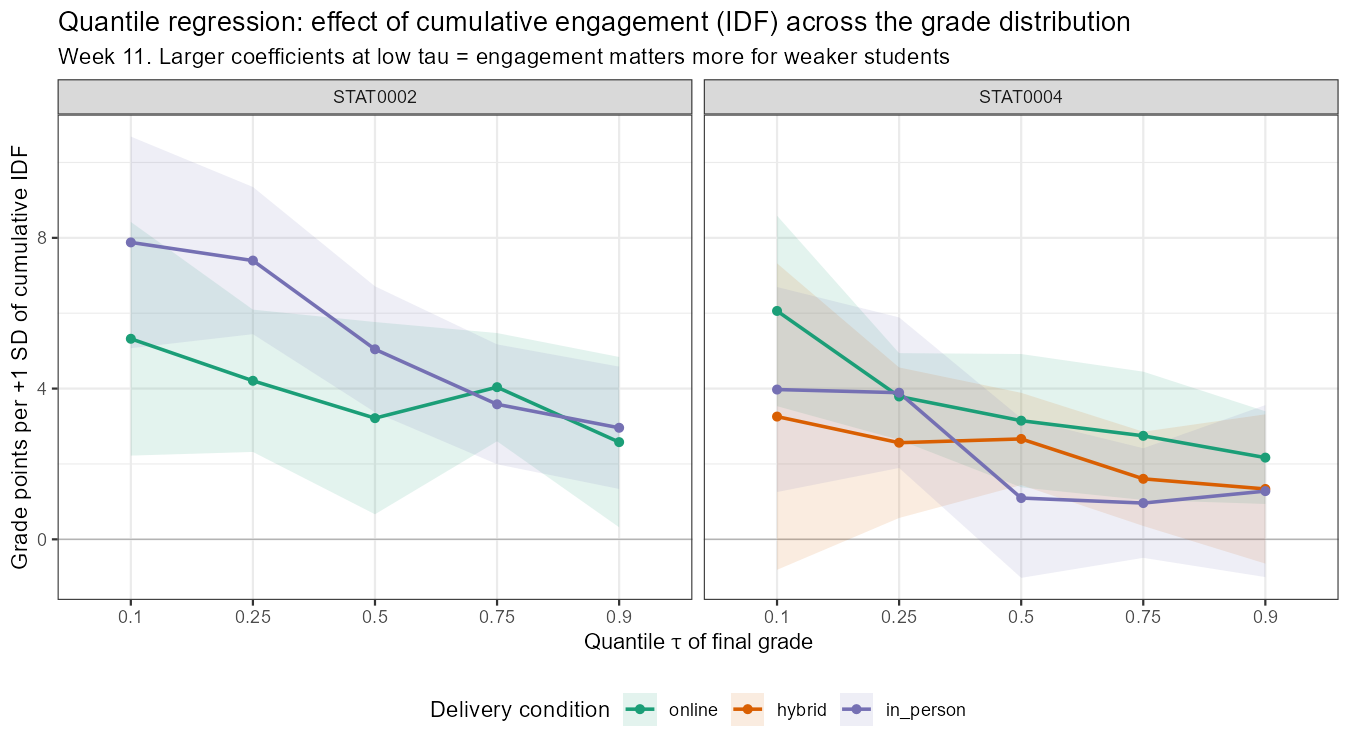
\includegraphics[width=0.92\textwidth]{11_quantile_idf.png}
\caption{Quantile-regression slopes of final grade on cumulative engagement across
the grade distribution. Slopes are steeper at $\tau=0.1$ than at the median in
every cohort, indicating that engagement variation is most consequential among
lower-performing students.}
\label{fig:quantile}
\end{figure}

Treating the bottom engagement quintile as an at-risk flag at the course midpoint,
STAT0002 cohorts identify roughly 38--47\% of students who ultimately score below
50\%, with AUC around 0.71--0.76, but precision remains modest (about
15--26\%). Many flagged students still pass. Figure~\ref{fig:earlywarn}
illustrates the familiar recall--precision trade-off reported in the primary
validation study.

\begin{figure}[H]
\centering
\includegraphics[width=0.95\textwidth]{08_recall_precision.png}
\caption{Recall and precision for the bottom engagement quintile across weeks.}
\label{fig:earlywarn}
\end{figure}

\subsection{Delivery-condition differences are descriptive and not conclusive}
Formal meta-analytic tests provide limited evidence that delivery condition
explains between-cohort variation in the engagement--grade relationship
(moderator $p > 0.87$ for all indicators; Table~\ref{tab:meta}). Weekly
correlations also appear broadly overlapping across online, hybrid and in-person
deliveries (Figure~\ref{fig:crossmod}). These patterns are consistent with a
relationship that is descriptively similar across the delivery periods represented
in the data. They do \emph{not}, however, establish that delivery mode is
irrelevant: because condition is confounded with academic year and cohort, the
design cannot separate delivery effects from differences in students, instructors,
assessment or pandemic-era context. External validation would be required before
concluding that the metric needs no recalibration in a new delivery format.

\begin{figure}[H]
\centering
\includegraphics[width=0.95\textwidth]{09_cross_module_weekly.png}
\caption{Weekly engagement--grade correlation by module and delivery condition.}
\label{fig:crossmod}
\end{figure}

\subsection{Breadth and promptness carry more signal than raw volume}
Because Frequency, Immediacy and Diversity are highly collinear, their individual
regression coefficients are difficult to interpret. The LMG decomposition provides
a clearer picture (Table~\ref{tab:importance}, Figure~\ref{fig:lmg}): Diversity
typically accounts for the largest share of explained variance (about 37\% on
average across cohorts), Immediacy is intermediate, and Frequency the smallest
(about 27\%). In plain terms, students who engage with a broader range of
resources and do so promptly tend to have stronger outcomes than would be
expected from activity volume alone.

\begin{table}[H]
\centering
\caption{LMG relative-importance shares (\%) by cohort.}
\label{tab:importance}
\small
\begin{tabular}{lccc}
\toprule
Cohort & Frequency & Immediacy & Diversity \\
\midrule
STAT0002 online    & 28 & 45 & 27 \\
STAT0002 in-person & 28 & 36 & 36 \\
STAT0004 online    & 23 & 32 & 45 \\
STAT0004 hybrid    & 31 & 32 & 38 \\
STAT0004 in-person & 25 & 33 & 42 \\
\bottomrule
\end{tabular}
\srcnote
\end{table}

\begin{figure}[H]
\centering
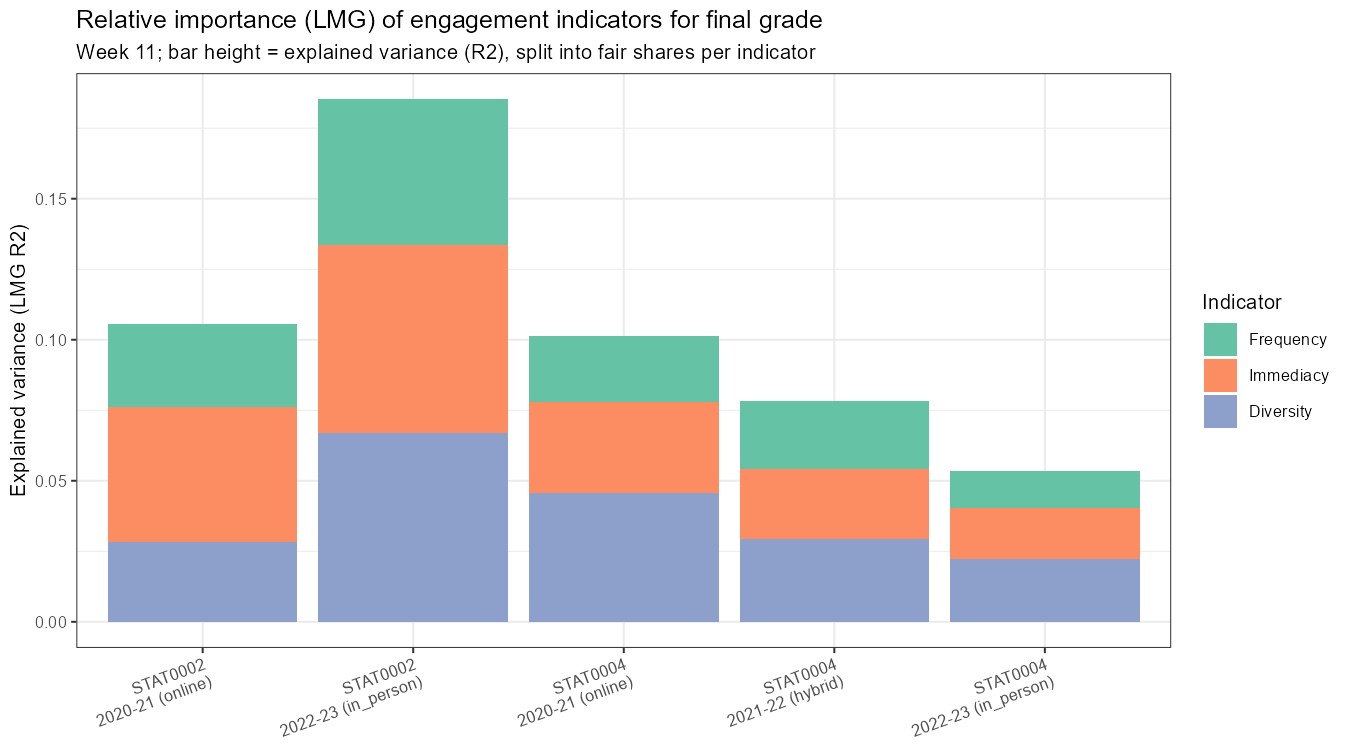
\includegraphics[width=0.9\textwidth]{13_lmg_importance.png}
\caption{LMG relative-importance shares for Frequency, Immediacy and Diversity by
cohort. Diversity and Immediacy typically account for more unique explained
variance than Frequency, suggesting that breadth and promptness matter more than
raw activity volume.}
\label{fig:lmg}
\end{figure}

\subsection{Engagement aligns more with individual assessment than group or peer assessment}
Engagement correlates more strongly with individually assessed components than
with group- or peer-marked work where both are available
(Figure~\ref{fig:component}). In STAT0002 in-person, the correlation with the
exam grade ($r=0.40$) is significantly larger than with peer-marking
($r=0.20$; Steiger $z=2.98$, $p=0.003$). Other component contrasts point in the
same direction but are not statistically significant. This supports the
interpretation that Moodle engagement reflects individual study behaviour more
faithfully than outcomes shaped by group dynamics or peer assessment.

\begin{figure}[H]
\centering
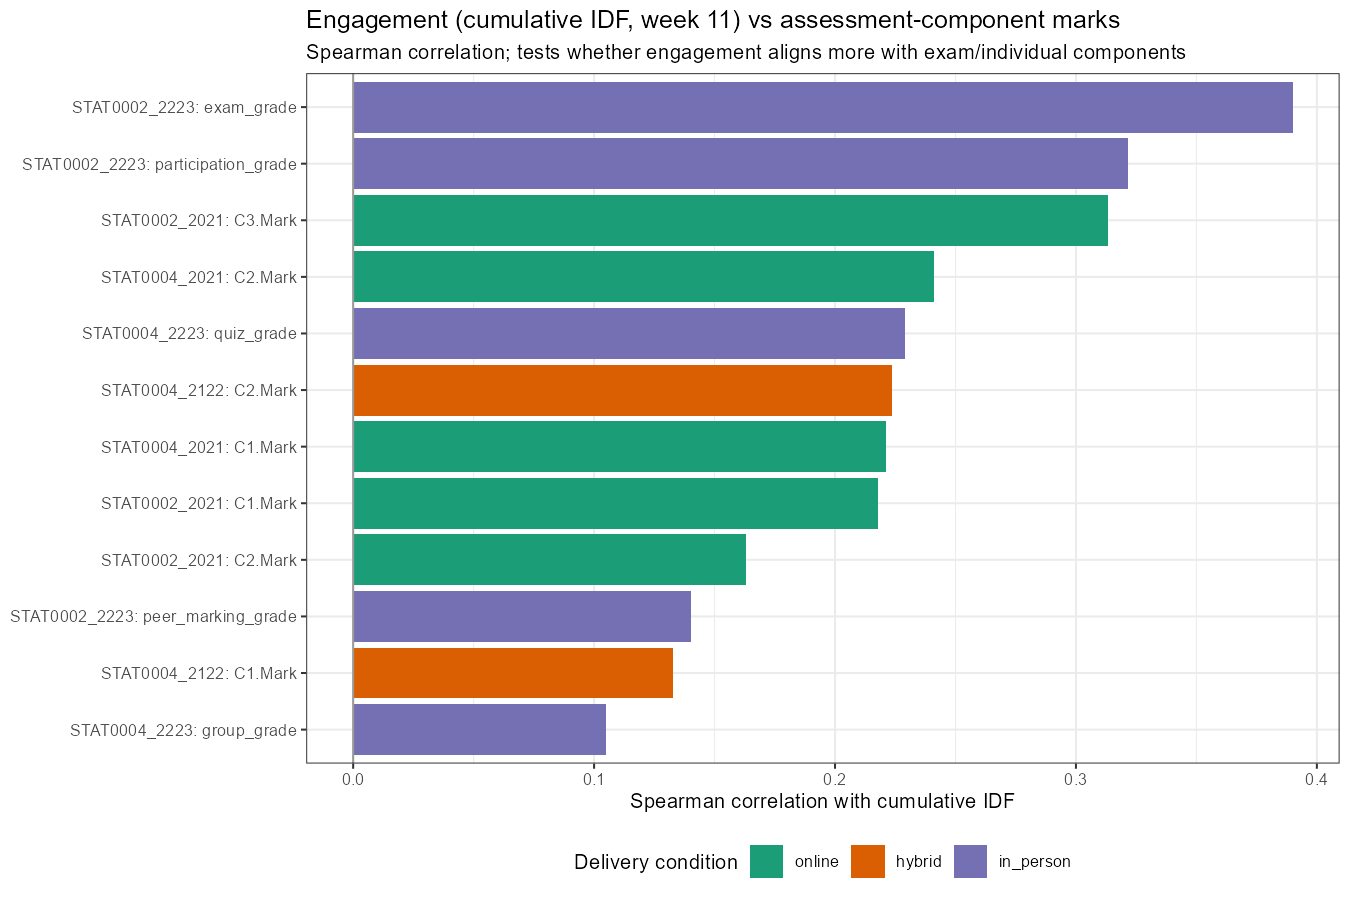
\includegraphics[width=0.92\textwidth]{14_component_correlations.png}
\caption{Engagement--assessment component correlations by cohort.}
\label{fig:component}
\end{figure}

\subsection{Temporal regularity adds diagnostic value}
Timing and regularity features add incremental explanatory power beyond F, I and
D in the STAT0002 cohorts, where engagement showed stronger alignment with
individual assessment components (Table~\ref{tab:temporal},
Figure~\ref{fig:temporal}). At week 6, the gain in $R^2$ is about 0.05 in both
STAT0002 deliveries ($p=0.003$ and $p=0.006$), but not statistically significant
in the STAT0004 deliveries. How regularly and promptly students work therefore
appears to carry additional information in STAT0002, beyond what the core composite
already captures.

\begin{table}[H]
\centering
\caption{Incremental $R^2$ from temporal features at week 6.}
\label{tab:temporal}
\small
\begin{tabular}{lcccc}
\toprule
Cohort & $R^2$ (F/I/D) & $R^2$ (full) & $\Delta R^2$ & $p$ \\
\midrule
STAT0002 online    & 0.091 & 0.143 & 0.052 & 0.003 \\
STAT0002 in-person & 0.156 & 0.213 & 0.057 & 0.006 \\
STAT0004 online    & 0.089 & 0.094 & 0.005 & 0.939 \\
STAT0004 hybrid    & 0.069 & 0.102 & 0.033 & 0.424 \\
STAT0004 in-person & 0.040 & 0.094 & 0.053 & 0.094 \\
\bottomrule
\end{tabular}
\srcnote
\end{table}

\begin{figure}[H]
\centering
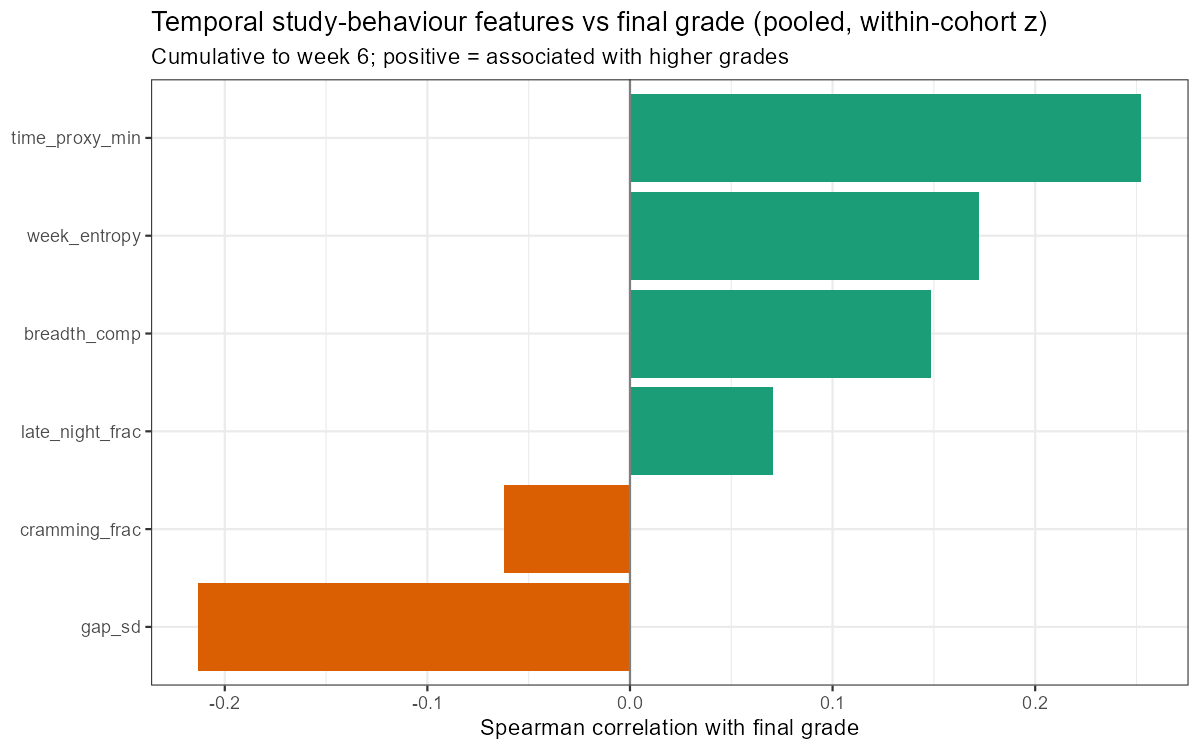
\includegraphics[width=0.92\textwidth]{16_temporal_feature_corr.png}
\caption{Temporal and regularity features correlated with final grade.}
\label{fig:temporal}
\end{figure}

\subsection{Engagement trajectories separate student outcomes}
Latent-class analysis of weekly cumulative IDF profiles favours a three-class
solution and identifies interpretable trajectory types: a low-steady group, a
high-steady group and a larger mid-variable group (Figure~\ref{fig:traj}).
Final grades differ markedly across classes (Kruskal--Wallis
$p = 2.6 \times 10^{-17}$). The high-steady class averages 72.9, compared with
63.2 for the low-steady class---a gap of about 9.7 grade points---and the
low-steady class contains the highest share of low performers (15.7\%). This is
among the strongest evidence in the report that sustained engagement patterns over
the term carry meaningful information about outcomes, beyond a single end-of-term
score.

\begin{table}[H]
\centering
\caption{Trajectory classes and grade outcomes ($N=1{,}290$).}
\label{tab:traj}
\small
\begin{tabular}{lccc}
\toprule
Class & $N$ & Mean grade & \%\,$<50$ \\
\midrule
Low-steady    & 439 & 63.2 & 15.7 \\
High-steady   & 165 & 72.9 & 2.4  \\
Mid-variable  & 686 & 68.3 & 5.5  \\
\bottomrule
\end{tabular}
\srcnote
\end{table}

\begin{figure}[H]
\centering
\begin{subfigure}{0.49\textwidth}
\centering
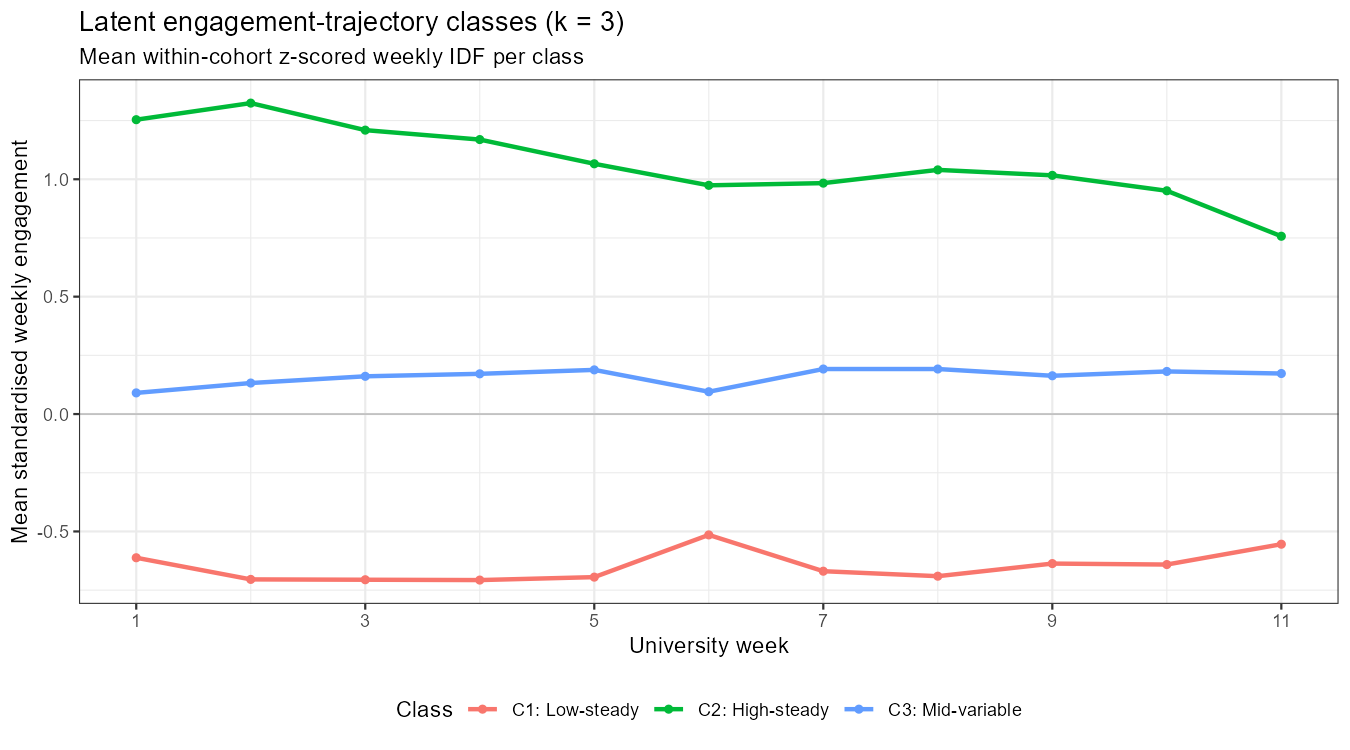
\includegraphics[width=\textwidth]{17_trajectory_shapes.png}
\caption{Trajectory shapes}
\end{subfigure}\hfill
\begin{subfigure}{0.49\textwidth}
\centering
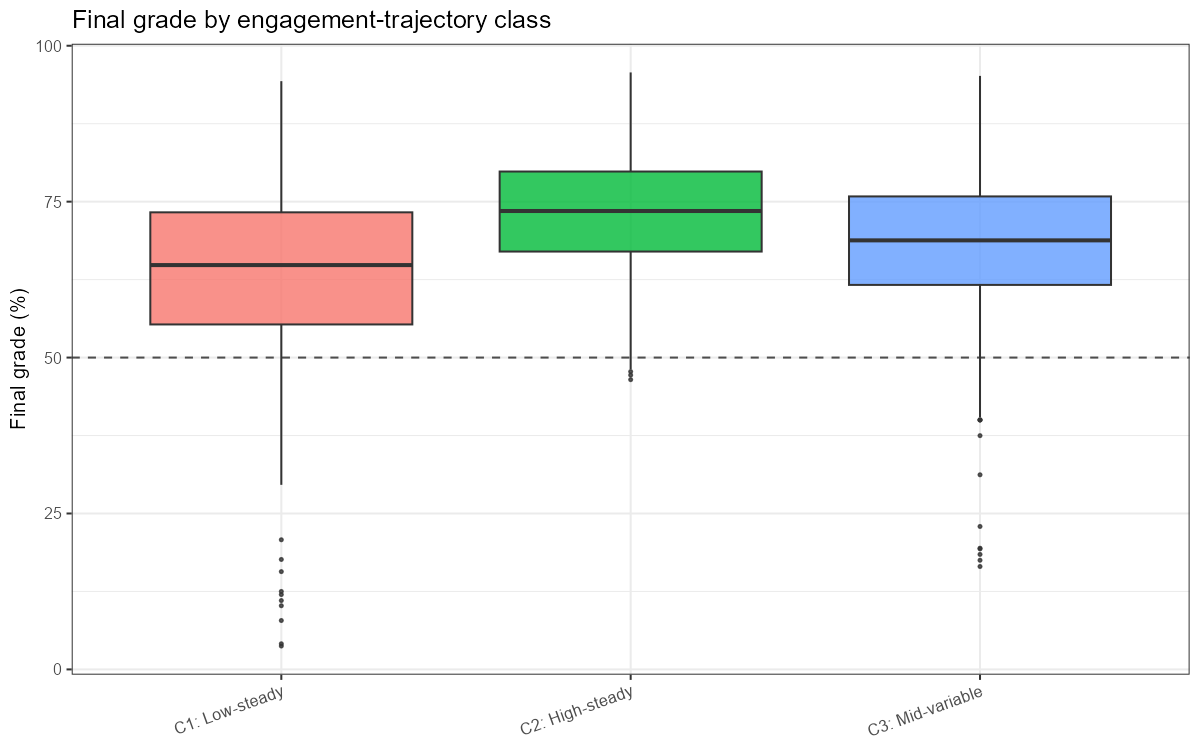
\includegraphics[width=\textwidth]{17_trajectory_grade.png}
\caption{Grades by class}
\end{subfigure}
\caption{Latent engagement trajectories (left) and final-grade distributions by
trajectory class (right). Three trajectory types---low-steady, high-steady and
mid-variable---separate outcomes by roughly 9.7 grade points between the
highest- and lowest-engagement profiles.}
\label{fig:traj}
\end{figure}

\subsection{Robustness checks}
The headline association is not an artefact of programme composition: adjusting
for degree programme changes the engagement slope by at most 14\%. Of 220 weekly
association tests across indicators and cohorts, 205 remain significant after
false-discovery-rate correction using the Benjamini--Hochberg procedure. Alternative bounded-outcome specifications agree
in sign with the main models in all five cohorts, and varying the at-risk
engagement threshold shifts recall and precision in the expected direction without
changing the overall interpretation.

\section{Discussion}
Taken together, the results support the chapter-aligned engagement metric as a
moderate but fairly stable observational proxy for academic performance in the
STAT0002 and STAT0004 cohorts studied here. The pooled association is positive in
every delivery, emerges early in most cohorts, and survives programme adjustment
and false-discovery-rate correction using the Benjamini--Hochberg procedure. This external validation on new module-year
contexts is broadly consistent with the primary findings of \citet{johnston2025},
while extending them through pooled inference and richer diagnostic analysis.

The most practically important pattern is that engagement appears especially
informative for lower-performing students. Quintile separation, quantile
regression and trajectory analysis all point in the same direction: students with
sustained low or narrow engagement profiles are disproportionately represented
among weaker grade outcomes. That does not mean the metric ``predicts failure''
with high accuracy---precision remains modest---but it does suggest value for
early, low-cost support aimed at students whose engagement profile indicates they
may be falling behind.

The diagnostic extensions add nuance that a single composite score alone would
hide. Raw session frequency is the least informative of the three core indicators
once collinearity is accounted for; breadth of resource use and promptness matter
more. Temporal regularity adds further information in STAT0002, and trajectory
shape separates outcomes as strongly as any single summary statistic. Engagement
also aligns more closely with individually assessed work than with peer- or
group-marked components, which strengthens the interpretation that Moodle logs
capture individual study effort rather than collaborative performance.

Delivery condition does not provide a simple explanation for differences across
cohorts. Descriptively, the engagement--grade relationship appears broadly similar
across the online, hybrid and in-person periods represented in the data, but the
design cannot disentangle delivery from year, cohort or curricular change. Module
design, assessment structure and how clearly Moodle resources map to chapters are
likely at least as important as the delivery label itself---a point reinforced by
the stronger alignment with individual assessment components in STAT0002 and the
weaker temporal-feature gains in STAT0004.

\section{Practical implications}
The metric is best understood as a transparent support tool rather than a
high-stakes predictor. It can be monitored from early in the term, explained to
students and instructors through its Frequency, Immediacy and Diversity
components, and used to prompt low-cost interventions such as nudges, check-ins or
invitations to office hours. Because many flagged students will ultimately pass,
it should be used as one signal among several, not as a basis for punitive action.

When engagement is low, the more useful question is often \emph{why} rather than
\emph{whether}: is the student behind the release schedule (Immediacy), touching
only a narrow set of resources (Diversity), or following a persistently low
trajectory? Those distinctions matter for how support is offered. Any operational
use in a new module or delivery context should be preceded by local validation,
especially where assessment design or resource labelling differs from the
cohorts studied here.

\section{Limitations}
Several limitations should be kept in view. Delivery condition is confounded with
academic year and cohort, so no causal inference about online, hybrid or in-person
delivery is possible. The analysis covers only two statistics modules and five
deliveries, limiting generalisability. Moodle logs capture online behavioural
engagement only; offline study is invisible. Final grades are imperfect outcome
measures, especially where group, peer or non-invigilated assessment contributes.
Low-performer counts are small in some cohorts, making early-warning metrics
unstable. The metric depends on consistent chapter labelling in Moodle. All
findings are associational, not causal. Frequency, Immediacy and Diversity are
highly collinear, so indicator-level interpretation requires appropriate methods.
Finally, external validation would be needed before operational deployment in new
contexts without recalibration.

\section{Conclusion}
This report provides secondary validation and diagnostic extension of an existing
chapter-aligned Moodle engagement metric across STAT0002 and STAT0004 cohorts.
Cumulative engagement is moderately and robustly associated with final grade,
especially among lower-performing students. The most informative signals are
breadth of resource use, promptness, temporal regularity and sustained trajectory
pattern, rather than raw activity volume alone. Delivery-condition comparisons
remain descriptive because condition is confounded with academic year and cohort.
The metric is therefore best understood as a transparent tool for early monitoring
and student support, not as a causal or high-stakes predictor of academic
outcomes.

\begin{thebibliography}{99}
\bibitem[Chong and Wong(2019)]{chong2019}
Chong, S., \& Wong, A. (2019). Proxy variables of online engagement on the learning
management system. \textit{International Journal of Learning and Teaching}, 296--300.

\bibitem[Conijn et al.(2017)]{conijn2017}
Conijn, R., Snijders, C., Kleingeld, A., \& Matzat, U. (2017). Predicting student
performance from LMS data: A comparison of 17 blended courses using Moodle LMS.
\textit{IEEE Transactions on Learning Technologies}, 10(1), 17--29.

\bibitem[Henrie et al.(2015)]{henrie2015}
Henrie, C.~R., Halverson, L.~R., \& Graham, C.~R. (2015). Measuring student
engagement in technology-mediated learning: A review. \textit{Computers \&
Education}, 90, 36--53.

\bibitem[Johnston et al.(2025)]{johnston2025}
Johnston, L.~J., Griffin, J.~E., Manolopoulou, I., \& Jendoubi, T. (2025). A
real-time metric of online engagement monitoring. \textit{arXiv preprint}
arXiv:2507.12162.

\bibitem[Lindeman et al.(1980)]{lindeman1980}
Lindeman, R.~H., Merenda, P.~F., \& Gold, R.~Z. (1980). \textit{Introduction to
bivariate and multivariate analysis}. Scott, Foresman.

\bibitem[Proust-Lima et al.(2017)]{proustlima2017}
Proust-Lima, C., Philipps, V., \& Liquet, B. (2017). Estimation of extended mixed
models using latent classes and latent processes: The R package lcmm.
\textit{Journal of Statistical Software}, 78(2), 1--56.

\bibitem[Steiger(1980)]{steiger1980}
Steiger, J.~H. (1980). Tests for comparing elements of a correlation matrix.
\textit{Psychological Bulletin}, 87(2), 245--251.

\bibitem[Viechtbauer(2010)]{viechtbauer2010}
Viechtbauer, W. (2010). Conducting meta-analyses in R with the metafor package.
\textit{Journal of Statistical Software}, 36(3), 1--48.
\end{thebibliography}

\end{document}
